% This is samplepaper.tex, a sample chapter demonstrating the
% LLNCS macro package for Springer Computer Science proceedings;
% Version 2.21 of 2022/01/12
%
\documentclass[runningheads]{llncs}
%
\usepackage[T1]{fontenc}
% T1 fonts will be used to generate the final print and online PDFs,
% so please use T1 fonts in your manuscript whenever possible.
% Other font encondings may result in incorrect characters.
%
\usepackage{graphicx}
% Used for displaying a sample figure. If possible, figure files should
% be included in EPS format.
%
% If you use the hyperref package, please uncomment the following two lines
% to display URLs in blue roman font according to Springer's eBook style:
%\usepackage{color}
%\renewcommand\UrlFont{\color{blue}\rmfamily}
%
\usepackage{amsmath}

\begin{document}
%
\title{An algorithm for finding the global extremum 
of a partially defined function\thanks{Supported by organization x.}}
%
%\titlerunning{Abbreviated paper title}
% If the paper title is too long for the running head, you can set
% an abbreviated paper title here
%
\author{Marina Usova\inst{1}\orcidID{0000-0002-0722-6884} \and
Konstantin Barkalov\inst{1}\orcidID{0000-0001-5273-2471}}
%
\authorrunning{M. Usova et al.}
% First names are abbreviated in the running head.
% If there are more than two authors, 'et al.' is used.
%
\institute{
Department of Mathematical Software and Supercomputing Technologies, Lobachevsky University, 603022 Nizhni Novgorod, Russia
\email{\{usova,konstantin.barkalov\}@itmm.unn.ru}}
%
\maketitle              % typeset the header of the contribution
%
\begin{abstract}
The paper discusses the problem of finding the global minimum of a function that may be partially defined in the search domain. The objective function may not be defined within some search regions due to the nature of the optimized object and of the simulation method (for example, numerical instability of the simulation method used). In some cases, these regions are known; but in most cases, the information about them is missing. The paper gives a description of a global search algorithm for solving such class of problems. Numerical experiments confirming the efficiency of the proposed algorithm were carried out.

\keywords{Lipschitz global optimization \and multiextremal functions \and hidden constraints \and dimensionality reduction.}
\end{abstract}
%
%
%
\section{Introduction}
Global optimization [...rus...] problems of finding the global (absolute) minima of multidimensional multiextremal functions. The possibility of building a reliable estimate of the global extremum in such problems is based principally on the availability of the \textit{a priori} known information on the problem to be solved allowing relating the possible values of the objective function to the known values in the points of search trials performed.

Often, such information is represented in the form of suggestion that the objective function $\phi$ satisfies the Lipschitz condition with a priori unknown constant $L$.

This suggestion can be interpreted (in the relation to the applied problems) as the reflection of a limited power generating the changes in the simulated system. At that, the objective function defined in the form of a "\textit{black box}"\ type functions as a rule is a non differentiable one, and each computation of its value in some point within a feasible domain may require considerable computational resources.

A number of efficient deterministic algorithms for solving the Lipschitz global optimization problems have been developed ~\cite{Jones2009,Birect2020,Sergeyev2017}. The comparisons conducted have shown the deterministic algorithms to overcome (in various criteria) the widespread nature-inspired algorithms ~\cite{Liberti2005,Sergeyev2018,Sovrasov2019} .

The present work continues the development of one of the efficient deterministic algorithms for solving the Lipschitz global optimization problems, namely the of the information-statistical algorithm of global search ~\cite{indexMethod,strongin1978,Strongin2000}. This algorithm suggests the solving of a multidimensional problem by means of its reduction to an equivalent one-dimensional optimization problem using the space-filling curves (Peano curves) ~\cite{Sergeyev2013}. 

Note that the use of complex mathematical models is natural in the optimization of complex real world objects that, as a consequence, increases the computation costs for searching the optimum Essentially. In last decades, the experts in the fields of optimization and parallel computations have proposed many methods for reducing the computation costs an speed-up of the algorithms related to solving the optimization problems appearing as well as to the numerical analysis of the original models [...ref???...].

However, a principally new problem in applications, namely the numerical instability of the models investigated in some (unknown a priori) regions in the ranges of the parameters’ variations became relevant recently. In such regions, one cannot perform the numerical modeling and compute the objective function values correctly. This phenomenon can be interpreted either as the presence of some hidden (unknown a priori) constraints In the problem or as a partial (limited) definition of the objective function in the search domain. In such a statement, the optimization problem becomes more complex essentially since the region of feasible parameters’ combinations is not defined in advance.

This paper presents the results in a new research direction related to the use of imputation\footnote{The term «imputation» in the paper is used following the established terminology in the field of machine learning related to the restoring of the missing data.} (restoring) of the objective function values in the course of the global search algorithm operation when solving the problems with partially defined objective functions. The approach proposed is based on an adoption of the computation rules of the global search algorithm. The efficiency of the approach proposed has been demonstrated numerically.

\section{Problem Statement}
In the general form, the global optimization problem can be formulated as follows:
\begin{equation}\label{eq1} 
\phi^*=\phi(y^* )=\min_{y \in D} \phi(y), D=\left\{ y \in R^N: a_i \leq y_i \leq b_i, a,b \in R^N,1 \leq i \leq N \right\},
\end{equation}
where $y=(y_1,y_2,...,y_N)$ - is the vector of the varied parameters, $D$ - is an $N$-dimensional hypercube, and $N$ –  is the dimension of the problem being solved.

Using the Peano curves mapping the interval $[0,1]$ onto the $N$-dimensional unitary hypercube unambiguously
$$
D=\left\{ y \in R^N: -2^{-1} \leq y_i \leq 2^{-1}, 1 \leq i \leq N \right\} = \left\{ y(x): 0 \leq x \leq 1 \right\},
$$
we can reduce the initial problem (\ref{eq1}) to a one-dimensional problem
\begin{equation}\label{eq2} 
\phi^*=\phi(y(x^* ))=\min_{x \in [0,1]} \left\{ \phi(y(x)) \right\},
\end{equation}
that allows applying efficient one-dimensional optimization algorithms for its solving.

We make the following assumptions on the objective function. 

First, the objective function may be multiextremal, nondifferentiable, and, moreo-ver, defined in the form of a "black box"\ (i. e. in the form of some subroutine, which entry the argument is supplied to, and the output is respective function value).

Second, each computing of the function in some point of the feasible region may require considerable computation resources.

Third, the objective function satisfies the Lipschitz condition
\begin{equation}\label{eq3} 
| \phi (y')-\phi (y'') | \leq L \| y'-y'' \|, y',y' \in D,
\end{equation}
where $L$ is the Lipschitz constant. The dimensionality reduction scheme using Peano curves is known to juxtapose the multidimensional problem with a Lipschitz objective function (\ref{eq1}) to problem (\ref{eq2}) with the one-dimensional objective function satisfying H{\"o}lder condition
\begin{equation}\label{eq4} 
| \phi (x')-\phi (x'') | \leq K \| x'-x'' \| ^{1/N}, x',x' \in [0,1],
\end{equation}
where $N$ is the dimensionality of the initial multidimensional problem and coefficient $K$ is related to the Lipschitz constant $L$ by the relation $K \leq 4L\sqrt N$ \cite{Strongin2000}.

Various versions of algorithms for solving the problems of such a class and respective theories of convergence are presented in \cite{Gourdin1996,Lera2015,strongin1978}.

Fourth, the objective function may be undefined in some regions of search domain $D$ (in particular cases, in one or in several points of this one).

From our experience in solving the applied optimization problems [...refs??...], we will assume the total volume of the non-computability regions to be a small fraction of the whole volume of the search domain $D$ (about 10-20\%)\footnote{When testing the algorithm, we have considered also more complex problem statements, which the volume of the non-computability region achieved 50-80\% in. The problems of this kind were solved by the algorithm proposed successfully as well but a large number of trials was required to solve the problem because the method attempted to explore the whole non-computability region. In this connection, in the rules of constructing the problems the experiments for the dimensionality $N=5$ were modified so that the non-computability region were located in the corners of the search domain only.}.

The last assumption makes the application of the classic information-statistical \textit{global search algorithm} \cite{indexMethod,strongin1978} or other Lipschitz optimization methods impossible and requires developing a modification for solving the problems with the objective functions, which are not defined everywhere.

\section{Solving Method}

\subsection{Description of Classic Global Search Algorithm}
Within the framework of the approach proposed, the information-statistical theory of global search is used for solving the problems (\ref{eq2}). The main idea of the algorithm is the use of the accumulated information to determine the next interval, which the absolute minimum is most probable to find within. The next trial point in this interval corresponds to the mathematical expectation of the minimum location.

Let us give more detailed description of the algorithm.

\subsubsection{Global search algorithm (GSA).} At every iteration of the global search a \textit{search trial} is executed. We will call a trial a computing the optimized function value  $\phi (x)$ from (\ref{eq2}). The first trial will be performed in the middle internal point $x^1 \in (0,1)$. The choice of the point $x^{k+1}, k \leq 1$ of the next $(k+1)^\text{th}$ trial is performed on the base of the following rules.

\paragraph{Rule 1.} Renumber (by the lower indices) the points $x^i, 1 \leq i \leq k$  of the previous trials in the ascending order by their coordinates i. e.
\begin{equation}\label{eq5} 
0=x_0 < x_1 < ... < x_i < ... < x_k=1
\end{equation}
and juxtapose these ones to the values $z_i=\phi (x_i), 1 \leq i \leq k$ computed in these points and to the indices $v_i=v(x_i)$ defined by the rule
\begin{equation}\label{eq6} 
v_i=v(x_i)=
  \begin{cases}
    -1 & {\quad \text{if } x_i \text{ is a boundary point,}}\\
    1  & {\quad \text{if } x_i \text{ is an internal point,}}
  \end{cases}
\end{equation}
the points $x_0=0$ and $x_{k+1}=1$ are introduced additionally (the values $z_0$ and $z_{k+1}$ are undefined) for convenience of the following notations.

\paragraph{Rule 2.} Compute current lower estimate
\begin{equation}\label{eq7} 
\mu = \max\left\{ \frac{|z_i-z_{i-1}|}{\Delta _i}, 2 \leq i \leq k \right\} , \Delta _i= \| x_i -x_{i-1} \| =(x_i-x_{i-1})^{1/N},
\end{equation}
of the unknown H{\"o}lder constant $K$ from (\ref{eq4}) for the reduced function $\phi(x)$ where $r, r>1$ is a parameter of the algorithm; if $\mu=0$ accept $\mu=1$.
\paragraph{Rule 3.} Determine the best current value of the objective function
\begin{equation}\label{eq8} 
z^*=\min \left\{ \phi (x_i): 1\leq i \leq k \right\}.
\end{equation}

\paragraph{Rule 4.} For each interval $(x_{i-1},x_i),1 \leq i \leq k+1$ compute the value $R(i)$ called a \textit{characteristic} of the interval according to the formula
\begin{equation}\label{eq9} 
R(x_i)=
  \begin{cases}
    \Delta _i+\frac {{(z_i-z_{i-1})}^2}{{(r \mu)}^2 \Delta _i} - 2 \frac {z_i+z_{i-1}-2z^*}{r \mu}, & {\quad  v(x_i)=v(x_{i-1})=1}\\
    2 \Delta _i-4 \frac {(z_i-z^*)}{r \mu}, & {\quad  v(x_{i-1})=-1, v(x_i)=1}\\
    2 \Delta _i-4 \frac {(z_{i-1}-z^*)}{r \mu}, & {\quad  v(x_{i-1})=1, v(x_i)=-1}
  \end{cases}
\end{equation}

\paragraph{Rule 5.} Select the interval $t$ with the largest value of characteristic $R(i):R(t)= \max_{1 \leq i \leq k+1} R(i)$.

\paragraph{Rule 6.} Perform the next trial in the middle point of the interval $(x_{t-1},x_t)$ if the indices of its end points are not the same i. e.
\begin{equation}\label{eq10} 
x^{k+1}=\frac {x_t+x_{t-1}}{2}, v(x_{t-1})\neq v(x_t),
\end{equation}
Otherwise, perform the next trial in the point
\begin{equation}\label{eq11} 
x^{k+1}= \frac {x_t+x_{t-1}}{2} -  \text{sign} {(z_t-z_{t-1})} \frac {{|z_t-z_{t-1}|}^N}{2r \mu ^N}, v(x_{t-1})=v(x_t).
\end{equation}

\textit{Stop criterion} of the algorithm, according to which the execution of the algorithm is terminated for current global optimization problem (\ref{eq2}) is the achievement of a predefined accuracy of the problem solution i. e. if the length of the interval $(x_{t-1},x_t)$ containing current point $x^{k+1}$ is less or equal to the predefined accuracy $\Delta _t \leq \varepsilon$ where $t$ is from Rule 5 and $\varepsilon >0$ is the predefined accuracy.

\subsection{ Approaches to the Reconstruction of the Objective Function Values }
The problem of not everywhere defined objective function described above is a partial analog of the long-standing missing data problem in Data Science. The origin of this problem may be, for example, the technical problems or assembling the data set from several sources with different sets of parameters.

It is worth noting that some machine learning algorithms can take into account and even restore the missing values in the data. For example, LightGBM has a regime of ignoring the missing values while XGBoost restores the data by means of the de-crease in the loss function when learning. Nevertheless, the majority of models can-not process the missing values and require the valid data without NaN or «missing» values. It makes this problem to be serious enough.

The experts in Data Science have proposed various approaches to the imputation (restoring) of the missing data:
\begin{itemize}
  \item Deleting of all cases, which have missing values of some variables (the last resort, the algorithm loses the access to the useful information contained in the on-missing observations’ values);
  \item Replacing any missing value with the average of the available values of the variable (doesn’t work with the qualitative variables, doesn’t account for the correlation of the data);
  \item Replacing by the most frequent value or by a constant (differs from the use of the median only by the ability to work with the qualitative parameters);
  \item Replacing the data using the method of $k$ nearest neighbors or kNN (unlike the former, accounts for the correlation between the parameters, sensitive to the fadeouts, computation costly);
  \item Multiple imputation by chained equations (MICE) – imputation of each value is performed not one but many times (allows understanding how reliable or unreliable is the value suggested);
  \item Imputation of the data using a deep learning (restores the missing values by means of training a neural network on the points, which all parameters are available for, computation costly for big data).
\end{itemize}

The absence of an universal algorithm and the necessity to find the most suitable methods for each particular problem are the common drawbacks of the approaches listed above.

For the imputation of the objective function values, one can consider, in general, a similar set of approaches, however, taking into account the Lipschitz condition and using the information-statistical theory. It allows selecting a universal algorithm fro this problem class. Next, the points, which the non-computability was found in are interpreted as the ones having the zero index, and (\ref{eq6}) is replaced by an extended formula
\begin{equation}\label{eq12} 
v_i=v(x_i)=
  \begin{cases}
    -1 & {\quad \text{if } x_i \text{ is boundary point}}\\
    1  & {\quad \text{if } x_i \text{ is internal point}}\\
    0  & {\quad \text{if } x_i \text{ is non-computability}}
  \end{cases}
\end{equation}

Let us describe various possible approaches to the implementation of the modification.

\subsubsection{The first approach.}To ignore the absence of the objective function value in the point. The characteristic of an interval with even a single non-computable point is computed from the length of the interval
\begin{equation}\label{eq13} 
R(i)=\Delta _i, \text{ if } v(x_i)=0 \text{ or } v(x_{i-1})=0.
\end{equation}

\begin{figure}
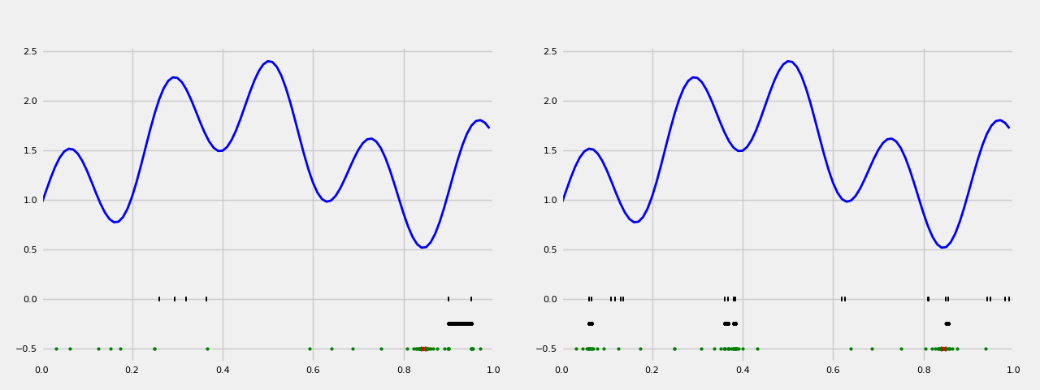
\includegraphics[width=\textwidth]{fig1.png}
\caption{Examples of the distributions of the search trials in the non-computability regions in the first approach to the imputation of the values} \label{fig1}
\end{figure}

A large number of excess trials after getting into the non-computability region due to a large value of the characteristic obtained according to (\ref{eq13}) is an essential draw-back of this approach.

\subsubsection{The second approach.} To ignore the absence of the objective function values in the point. The characteristic of the interval with two non-computable point or with one non-computable point and one boundary point is computed from the interval multiplied by a reducing constant
\begin{equation}\label{eq14} 
R(i)={(1- \frac {1}{r})}^N \Delta _i,
\end{equation}
if $v(x_i)=v(x_{i-1})=0$ or $v(x_i)=0$ and $v(x_{i-1})=-1$ or $v(x_i)=-1$ and $v(x_{i-1})=0$.
The characteristic of the interval with one non-computable point and one computable point is calculated according to the rules of operation with the boundary interval
\begin{equation}\label{eq15} 
R(i)=2\Delta _i-4 \frac {(z_i-z^*)}{r \mu},\text{ if } v(x_{i-1})=-1  \text{ or } v(x_{i-1})=0, v(x_i)=1,
\end{equation}
\begin{equation}\label{eq16} 
R(i)=2\Delta _i-4 \frac {(z_{i-1}-z^*)}{r \mu},\text{ if } v(x_{i-1})=1, v(x_i)=-1 \text{ or } v(x_i)=0.
\end{equation}

\begin{figure}
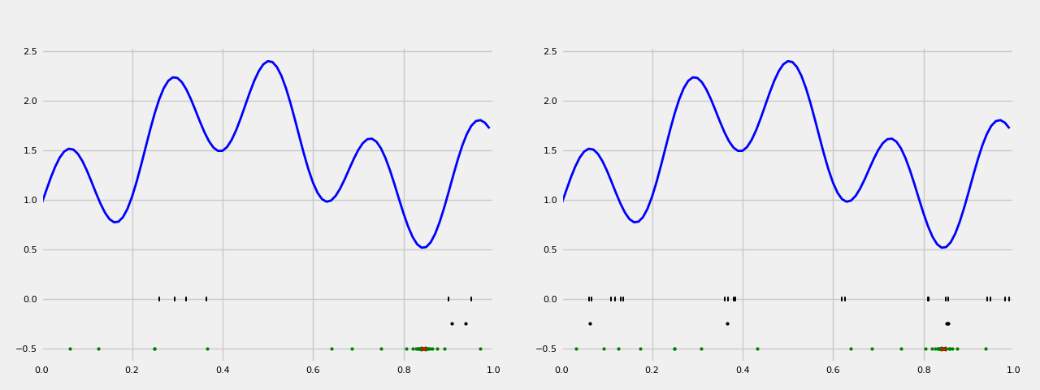
\includegraphics[width=\textwidth]{fig2.png}
\caption{Examples of the distributions of the search trials in the non-computability regions in the second approach to the imputation of the values} \label{fig2}
\end{figure}

This approach resolves partly the problems of the first approach outlined above. However, it doesn’t solve the problem of excess trials and requires a considerable increasing of the parameter $r$ for more complex test problem. The examples for the one-dimensional problems using the first two approaches are presented in ~\ref{fig1} and ~\ref{fig2} where the trials falling into the region with the undefined values are marked by the black points and the computable points of the search domain – by the green ones. 

\subsubsection{The third approach.} To restore the objective function values in the points of the intervals with two non-computable points as the averages of the neighbor points and to apply corresponding computation rule from formula (\ref{eq9}) assuming the points to be computable ones. If the neighbor points are non-computable as well, to use formula (\ref{eq14}). In the case of an interval with one non-computable point, to apply formulae (\ref{eq15}) and (\ref{eq16}).
\begin{figure}
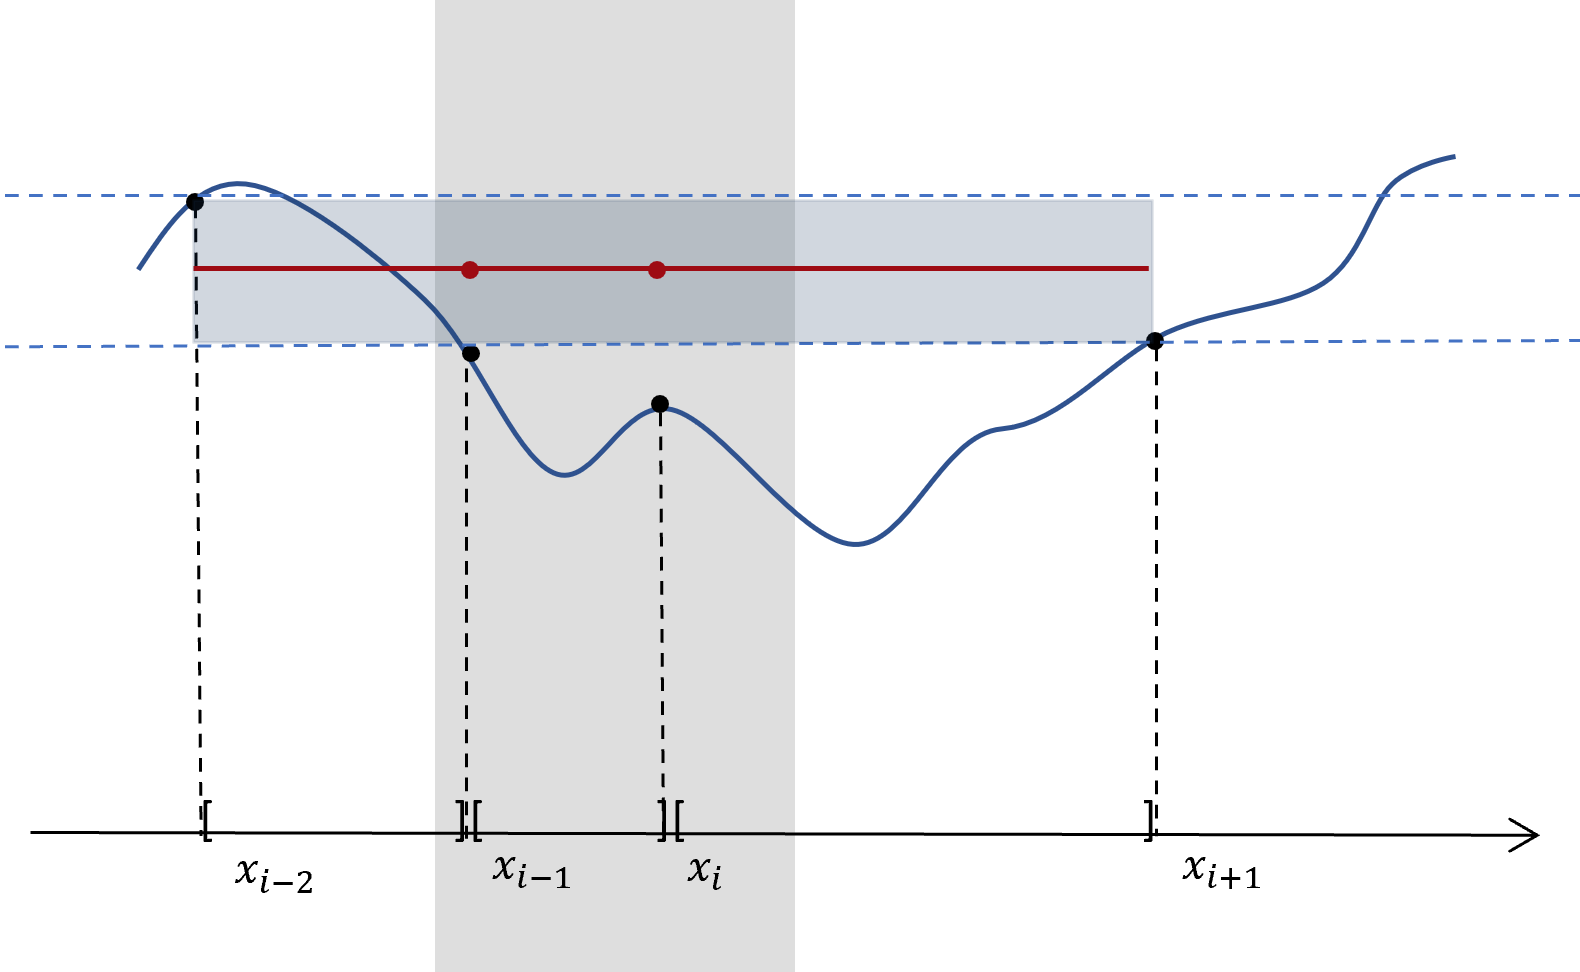
\includegraphics[width=\textwidth]{fig3.png}
\caption{Imputation of the non-computable values by the averages of the neighbor points. Approach \#3} \label{fig3}
\end{figure}

Essential drawbacks of this approach are not utilizing the information on the coordinates aw well as seldom executing the computation rule added because of searching the substituting values among the nearest neighbors only.

\subsubsection{The fourth approach.} To restore the objective function values in the points for the intervals with two non-computable points as the averages of the nearest computable points taking into account the location coordinates i. e.
\begin{equation}\label{eq17} 
\tilde{z}(x)=z'+ \text{sign}(z''-z') \frac {|z''-z'| \cdot \| x-x' \|}{\| x''-x' \|},
\end{equation}
where $z'$ and $z''$ are the objective function values in the computable points $x'$ and $x''$  nearest to the interval.
The rest of the approach is identical to the third one. Formula (\ref{eq14}) in this case will be applied when the non-computable region is located near the boundary point only.
\begin{figure}
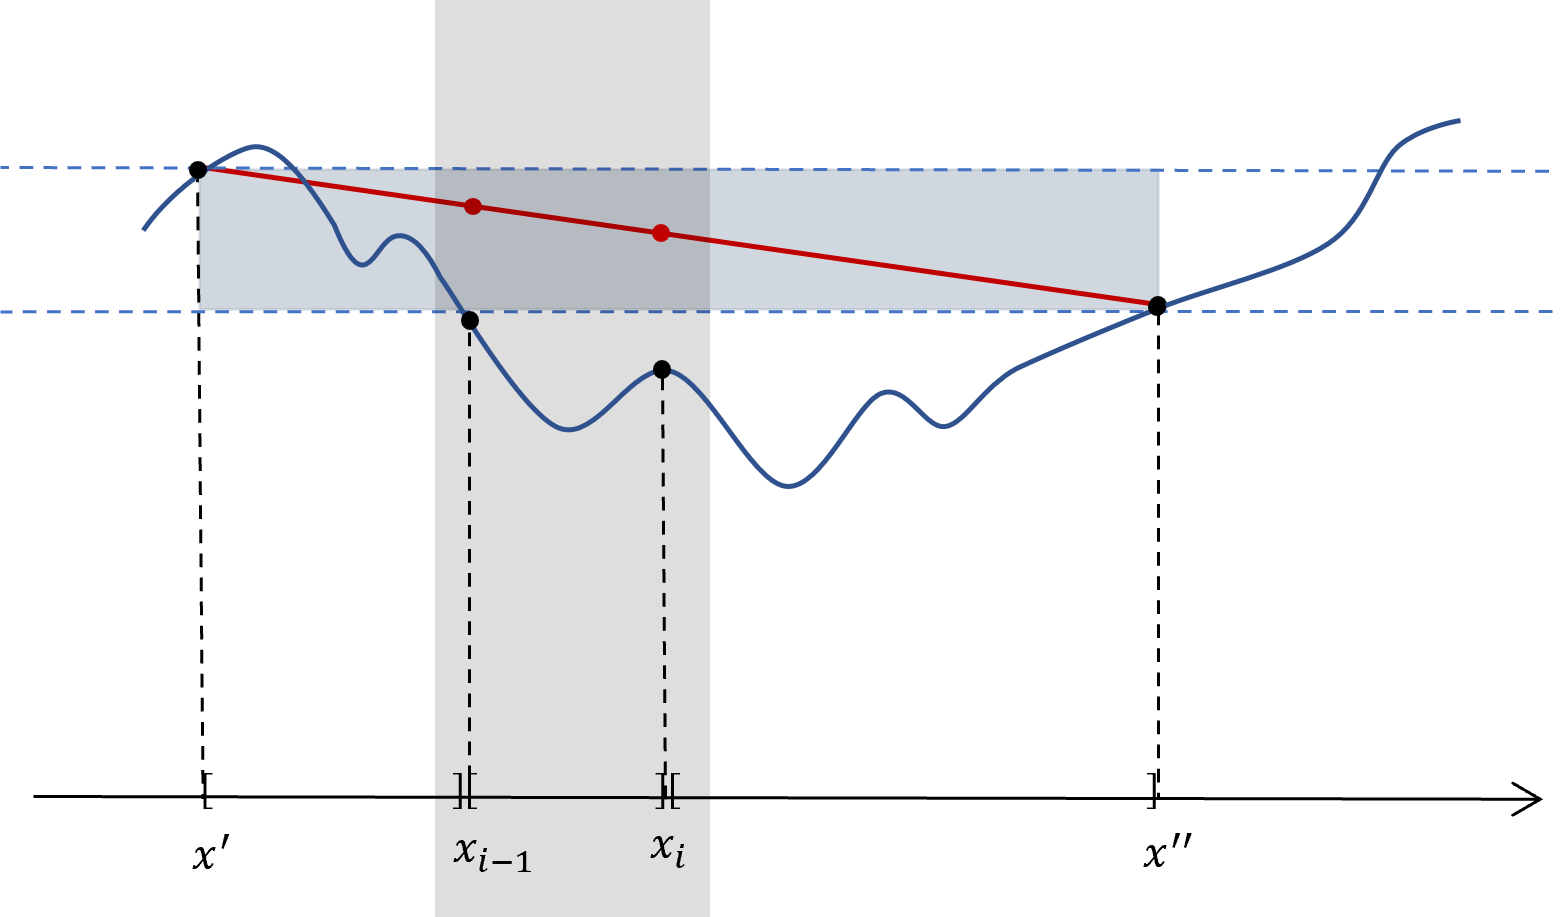
\includegraphics[width=\textwidth]{fig4.png}
\caption{Imputation of non-computable values by averages of the neighboring points. Approach \#4} \label{fig4}
\end{figure}
\begin{figure}
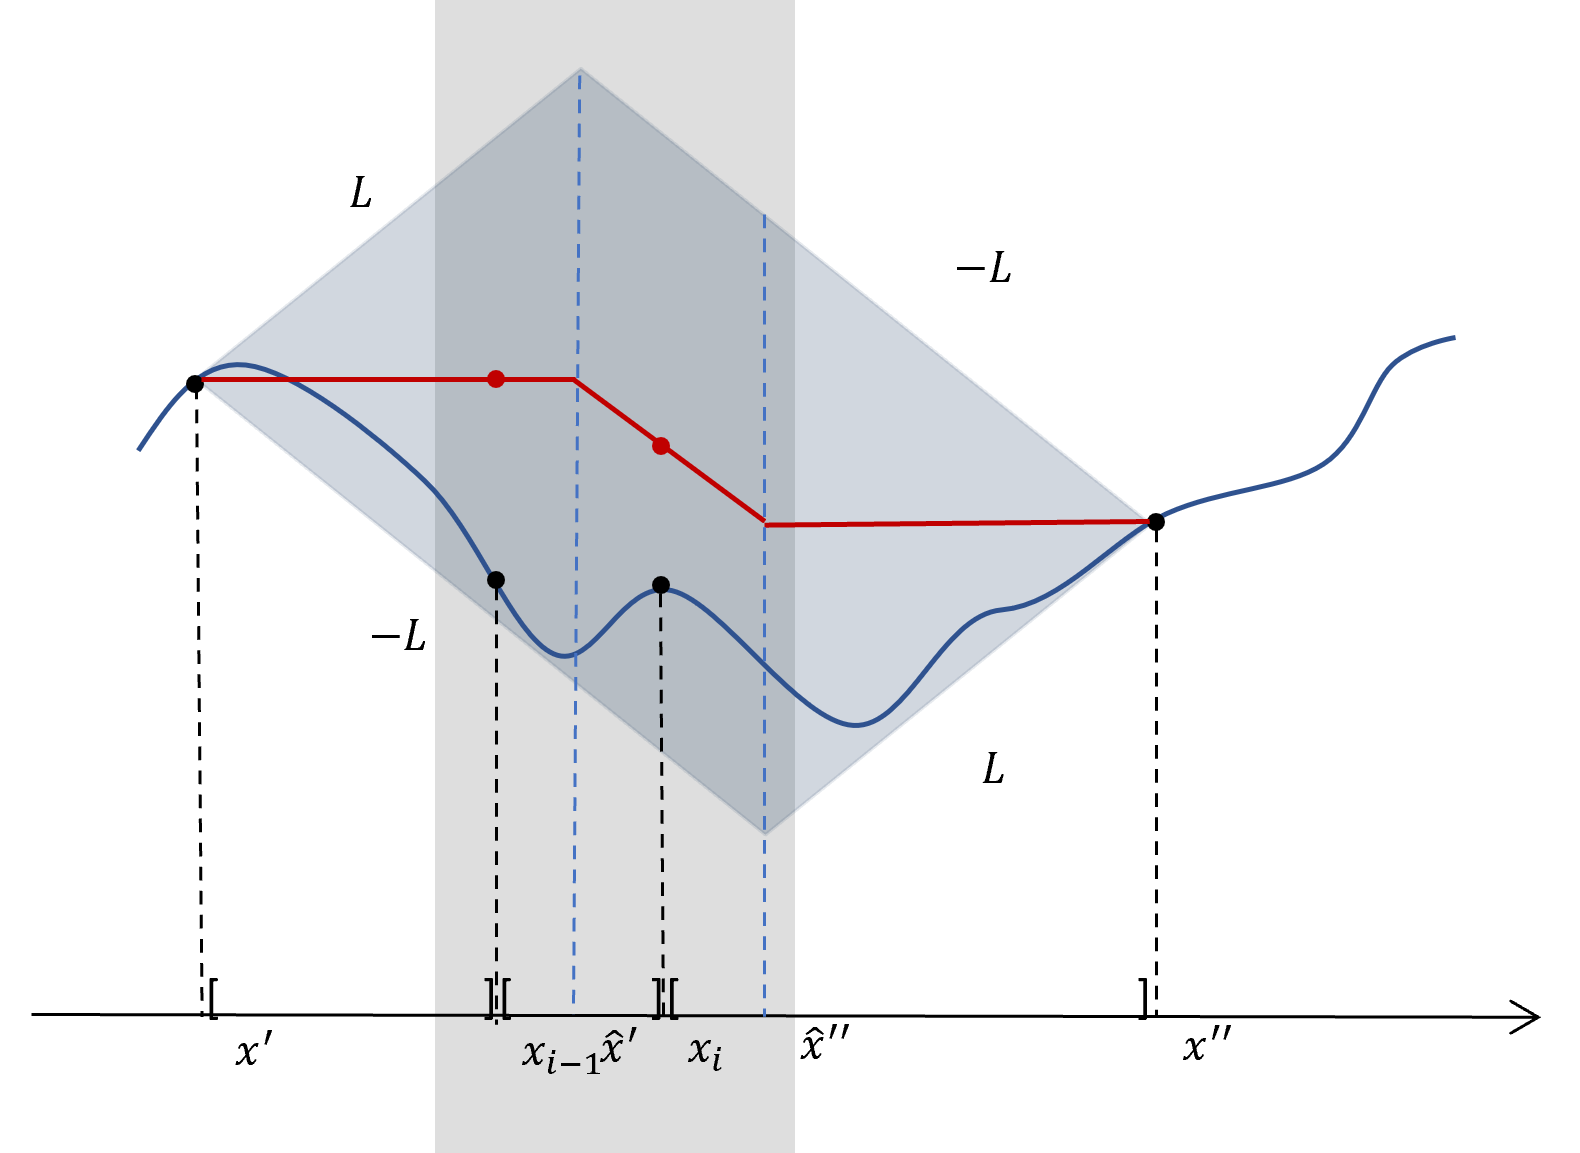
\includegraphics[width=\textwidth]{fig5.png}
\caption{Imputation of non-computable values by averages of the minorant and the majorant. Approach \#5} \label{fig5}
\end{figure}

\subsubsection{The fifth approach.} To utilize the search information and the suggestions on the function form most completely, one can restore the objective function values in the points taking onto account the H{\"o}lder condition.
\paragraph{Step 1.} Find the end points of the crossing of majorant and minorant
\begin{equation}\label{eq18} 
\hat{x}',\hat{x}''=\frac {x'+x''}{2}\pm \text{sign}(z''-z')\cdot \frac {1}{2r} \cdot {\left(\frac {z''-z'}{\mu}\right)}^N,
\end{equation}
\paragraph{Step 2.} Restore the objective function values according to the rule
\begin{equation}\label{eq19} 
\tilde{z}(x)=
  \begin{cases}
    z', & {\quad x \leq \hat{x}',}\\
    \frac {z'+z''}{2}- \frac {r \mu}{2} (\| x - x' \| + \| x - x'' \|), & {\quad \hat{x}' < x < \hat{x}'',}\\
    z'',  & {\quad x \geq \hat{x}''.}
  \end{cases}
\end{equation}
This rule can be interpreted as an average value of the minorant and the majorant for a function satisfying the H{\"o}lder condition. Let us give the description of the modification of the global search algorithm in the case of not everywhere computable function based on this approach.

\subsubsection{Description of the modification.} The algorithm remains the same with an introduction of the following minor additions in the computing formulae in the case of falling into the non-computable search regions:
\begin{enumerate} 
  \item The index $v_i=v(x_i)$ is determined by the formula (\ref{eq12}).
  \item When computing current lower estimate of the H{\"o}lder constant $K$ in formula (\ref{eq7}), use the intervals with two computable points only.
  \item The best current objective function value is determined for different values of the index
\begin{equation}\label{eq20} 
z_v^*=
  \begin{cases}
    -\varepsilon _r, & {\quad v=0 ,}\\
    \min \left\{ \phi (x_i): v(x_i)=1, 1 \leq i \leq k \right\}, & {\quad v=1 ,}
  \end{cases}
\end{equation}
where $\varepsilon _r$ is a parameter of the method.

  \item For each interval $(x_{i-1}, x_i), 1 \leq i \leq k+1$, the computing of the characteristic $R(i)$ is performed according to the following computing formulae.
      \begin{itemize} 
        \item \textit{Case 1.} For the intervals with \textbf{two computable points} or with \textbf{one computable point and one boundary point}, apply the classic rules of global search algorithm
\begin{equation}\label{eq21} 
R(i)=
  \begin{cases}
     \Delta _i+\frac {{(z_i-z_{i-1})}^2}{{(r \mu)}^2 \Delta _i} - 2 \frac {z_i+z_{i-1}-2z_1^*}{r \mu}, & {\quad  v(x_i)=v(x_{i-1})=1}\\
    2 \Delta _i-4 \frac {(z_i-z_1^*)}{r \mu}, & {\quad  v(x_{i-1})=-1, v(x_i)=1}\\
    2 \Delta _i-4 \frac {(z_{i-1}-z_1^*)}{r \mu}, & {\quad  v(x_{i-1})=1, v(x_i)=-1}
  \end{cases}
\end{equation}
        \item \textit{Case 2.}  For the intervals with \textbf{one boundary point and one non-computable point}, perform the imputation of the values for the non-computable point based on the neighbor computable point and apply the formula
\begin{equation}\label{eq22} 
R(i)=
  \begin{cases}
    2 \Delta _i-4 \frac {(z_{i+1}-z_0^*)}{r \mu}, & {\quad  v(x_{i-1})=-1, v(x_i)=0}\\
    2 \Delta _i-4 \frac {(z_{i-2}-z_0^*)}{r \mu}, & {\quad  v(x_{i-1})=0, v(x_i)=-1}
  \end{cases}
\end{equation}
        \item \textit{Case 3.} For the intervals with \textbf{one non-computable and one computable point}, perform the imputation of the value for the non-computable point based on the neighbor com-putable point and apply the formula
\begin{equation}\label{eq23} 
R(i)=
  \begin{cases}
     \Delta _i+\frac {{(z_i-z_{i-2})}^2}{{(r \mu)}^2 \Delta _i} - 2 \frac {z_i+z_{i-2}-2z_0^*}{r \mu}, & {\quad  v(x_{i-1})=0, v(x_i)=1}\\
     \Delta _i+\frac {{(z_{i+1}-z_{i-1})}^2}{{(r \mu)}^2 \Delta _i} - 2 \frac {z_{i+1}+z_{i-1}-2z_0^*}{r \mu}, & {\quad  v(x_{i-1})=1, v(x_i)=0}
  \end{cases}
\end{equation}
        \item \textit{Case 4.}. For the intervals with \textbf{two non-computable points}, perform the imputation of the values for the non-computable points based on the rule (\ref{eq19}) and apply the formula
\begin{equation}\label{eq24} 
R(i)=\Delta _i+\frac {{(\tilde{z}_i-\tilde{z}_{i-1})}^2}{{(r \mu)}^2 \Delta _i} - 2 \frac {\tilde{z}_i+\tilde{z}_{i-1}-2z_1^*}{r \mu}, v(x_{i-1})=v(x_i)=0
\end{equation}
        \item \textit{Case 5.} In the case when any imputation is impossible, use the formula
\begin{equation}\label{eq25} 
R(i)=\Delta _i \cdot {\left( 1-\frac {1}{r} \right)}^N+z_0^*.
\end{equation}
    \end{itemize} 
  \item If several intervals have equal characteristics, prefer the computable interval with the lowest number.
  \item If the best interval appears to be the one with two non-computable points, perform the next trial in the middle point of the interval.
\end{enumerate}

\subsection{Results of Numerical Experiments}
The numerical experiments were carried out using a computer with Intel® Core™ i7-10750H CPU @ 2.60GHz 2.59 GHz using the developed software package implementing the modification described in Section 3. To generate a series of problems, GKLS generator described in \cite{Gaviano2003} was used. It allows generating the multiextremal oprimization problems with the properties known in advance. These problems were appended with the non-computable regions of various kinds.

Each series of experiments consisted of 100 GKLS problems with everywhere computable objective function (the classic GKLS problems), 100 problems with the non-computabilities at the boundaries of the search domains, and 100 problems with non-computability regions defined randomly.

In the first series of experiments, the correctness of the modification operation was checked and the features of executing the trials in the non-computability regions were revealed. The problems of the dimensionality $N=2$ were used in the experiment. The reliability parameter was set to $r=5.5$, the precision $\varepsilon=0.01$. The results of experiments are presented in Tab.~\ref{tab1}.

\begin{figure}
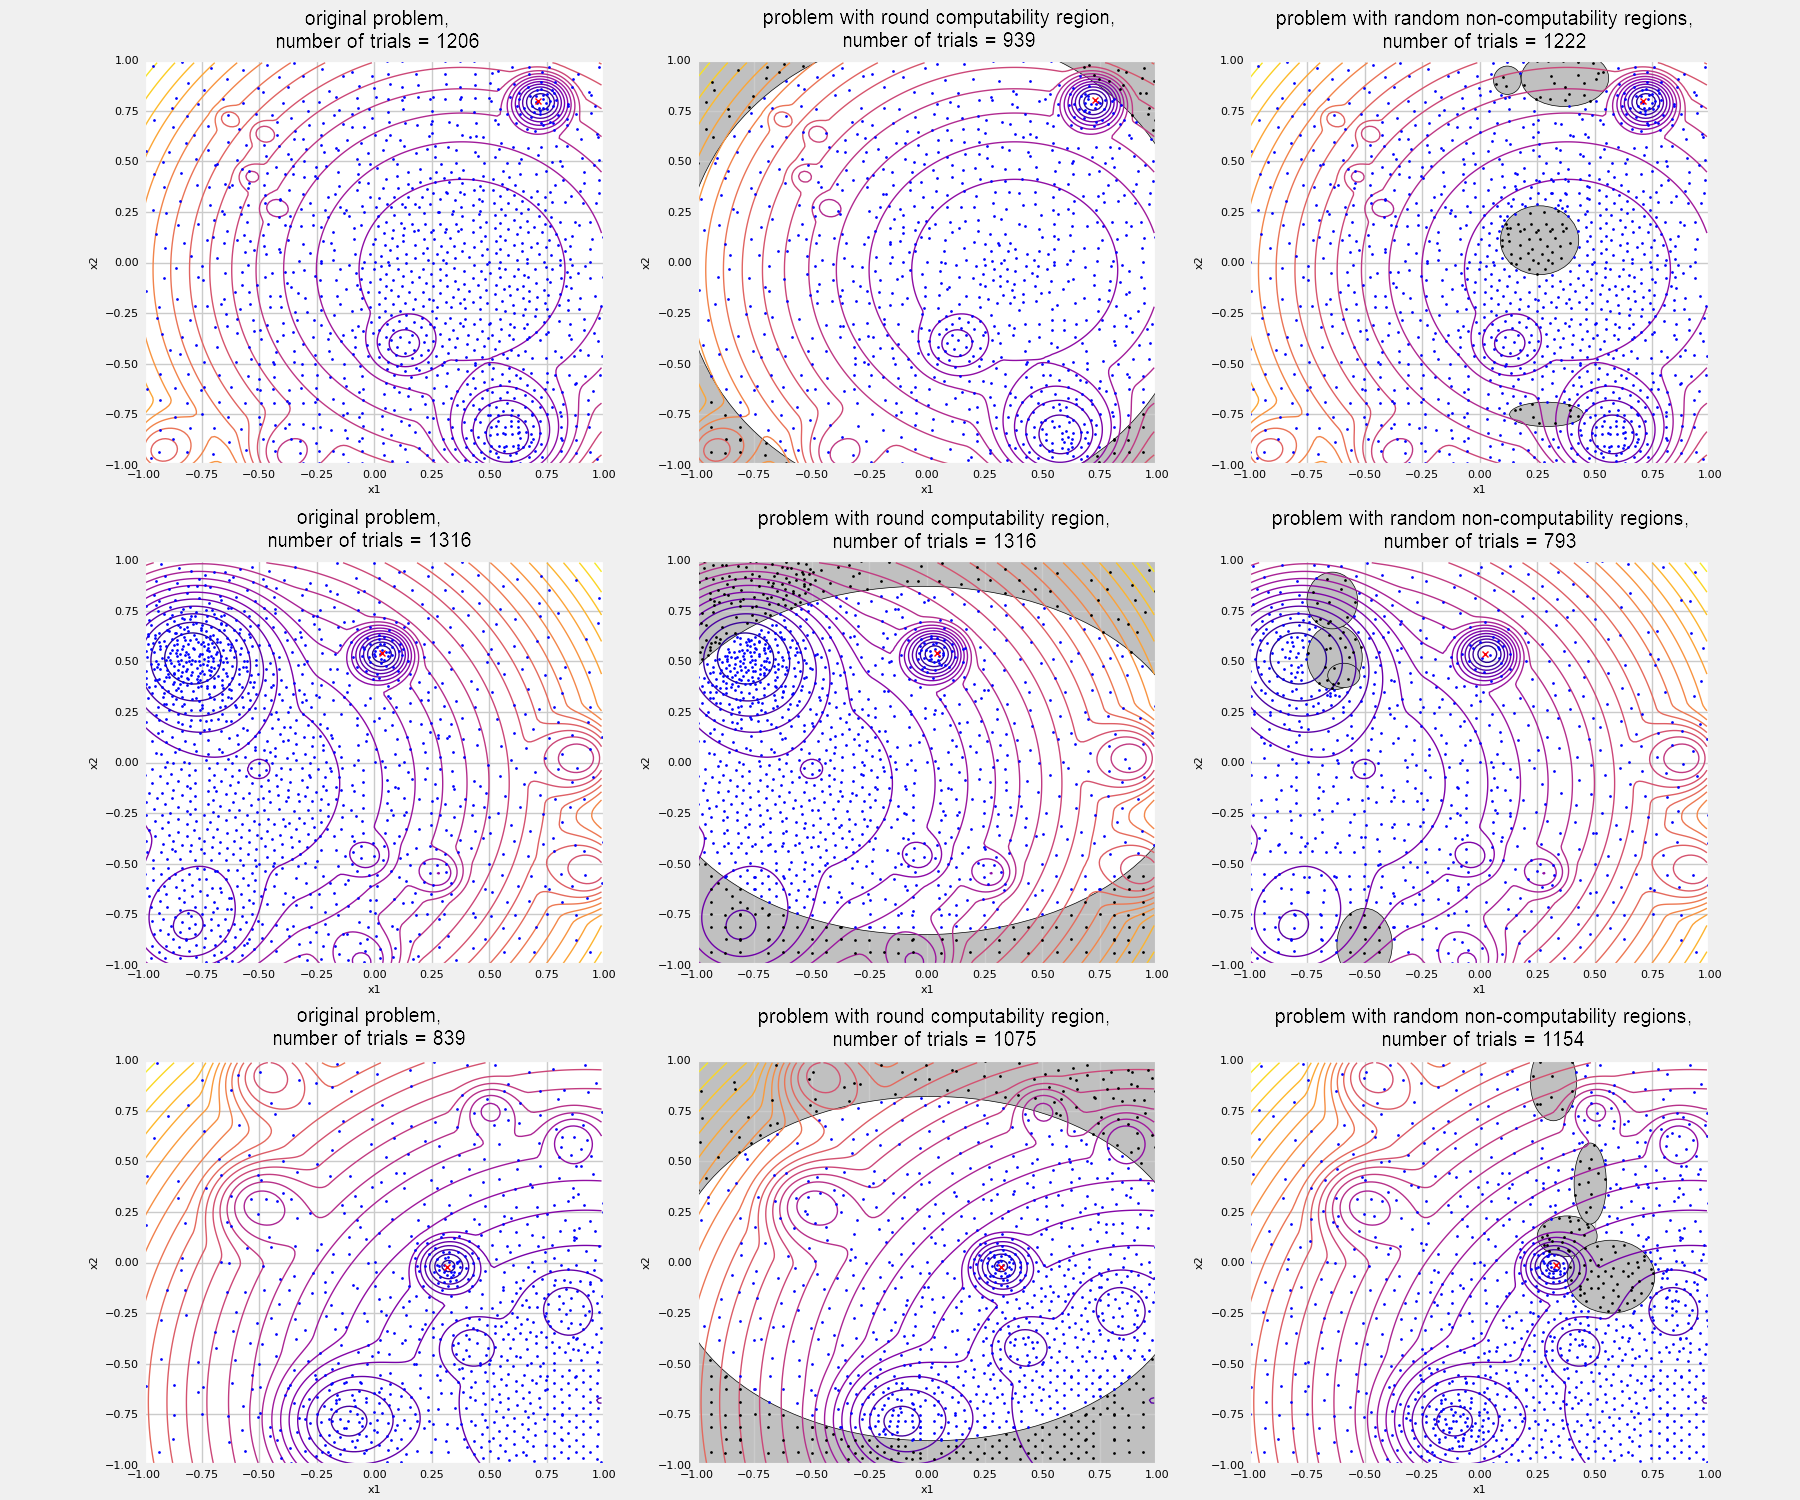
\includegraphics[width=\textwidth]{fig6.png}
\caption{Examples of problems \#\# 19, 25, and 35 from the first series of experiments} \label{fig6}
\end{figure}

Fig.~\ref{fig6} presents the examples of the modification operation with several problems of the series. The trials inside the computable regions are denoted by the blue points in the figures, the global minima of the problems – by the red points, and the points of trials performed inside the non-computability regions – by black. Also, the non-computability regions are filled with grey for clarity.

Since the modification works with the classic GKLS problem series according to the base global search algorithm, one can compare it with the classic GSA. Thus, the general behavior of GSA was preserved for the modification, and the same regions of trials’ densification near the local minima were observed that can be explained by the realization of the classical computation rules (\ref{eq21}) in most cases. One can see in Tab.~\ref{tab1} that the number of trials executed inside the non-computable regions is small. Total number of trials for the classic problems and for the problems with non-computable regions are comparable, the method doesn’t perform excess iterations in the non-promising regions due to the computing formulae utilizing the information on the nearest computable points.

\begin{table}
\caption{Comparison of the efficiencies of the algorithm modification with the classic version of the global search algorithm on GKLS problems}\label{tab1}
\begin{tabular}{|l|c|c|c|}
\hline
 &  classical  &  round district  &  random district  \\
\hline
Average number of iterations & 781,66	& 854,91 & 839,03 \\
Average number of non-computability & - & 185,79 & 42,31 \\
Number of solved problems & 100 / 100 & 100 / 100 & 100 / 100\\
\hline
\end{tabular}
\end{table}

The use of rule (\ref{eq25}) forms a grid of trials inside the non-computability regions that is visible clearly for Problem \#35. At that, the trial points are denser at the boundary of the non-computable region close to potential minimum when attempting to approach this one from different sides due to the computational rules (\ref{eq22})-(\ref{eq24}) that was observed in all problems presented as the examples. 

100\% of the problems were solved. However, for the series with the boundary non-computability region, the value of parameter $r=6.0$ was required to solve one problem, for the series with the random regions – soving of two problems with given value of parameter $r$.

In the second series of experiments, the problem series of various dimensionalities were solved. In the experiments with the problems of the dimensionality $N=4$, the reliability parameter was set to $r=4.5$, the precision $\varepsilon=0.02$. The global minimum was considered to be found if the algorithm generates a trial point inside the $\varepsilon$-nearness of the global minimum. The results of the experiments are presented in Tab.~\ref{tab2}.

\begin{table}
\caption{Problem series of various dimensionalities}\label{tab2}
\begin{tabular}{|l|l|c|c|c|}
\hline
 N &  Task type & Average num. of iters & Average num. of non-comput. & Solved problems \\
\hline
$3$ & classical & 12251,11 & - & 100 / 100 \\
$ $ & round & 12201,78 & 4763,57 & 100 / 100 \\
$ $ & random & 12210,71 & 63,39 & 100 / 100 \\
\hline
$4$ & classical & 25144,46 & - & 100 / 100 \\
$ $ & round & 29840,32 & 15004,37  & 100 / 100 \\
$ $ & random & 25287,49 & 26,43 & 100 / 100 \\
\hline
$5$ & classical & 56725,95 & - & 100 / 100 \\
$ $ & round & 47840,09 & 24109,19 & 100 / 100\\
$ $ & random & 57874,76 & 82,57 & 100 / 100\\
\hline
\end{tabular}
\end{table}

According to the results of the experiments, the method resolves successfully the occasional falls into the non-computability regions scattered inside the search domain randomly whereas in the case of large boundary regions it tries the execute a complete investigation without executing too many excess trials.

\subsection{Conclusions}
In the present work, the problem of finding the global minimum of a computation-costly "black box"\ function was considered. As compared to the traditional formulation used in the global optimization, the problem considered has an important differ-ence: the objective function may be undefined in some regions of the search domain (in particular, in one point or in several ones). The appearing of such a problem statement is caused by a frequent problem of numerical instability of the models investigated in the applied problems.

The main problem is the impossibility to identify the non-computability regions in advance in most cases. In fact, the region of feasible combinations of parameters is undefined a priori. This phenomenon can be interpreted as the presence of additional hidden constraints in the problem.

The problem investigated in the present work echoes to problem of missing data existing in Data Science for a long time. As a solution, the experts in the field have proposed various approaches to the imputation (restoring) of the missing values. These ideas have found their reflection in the development of the new method.

The applicability of already existing approaches appended with various variants to account for the Lipschitz condition was investigated. As a result, a universal efficient algorithm for solving the problems of this class has been developed. The algorithm constructed is a development of one of efficient deterministic method of solving the Lipschitz global optimization problems, namely information-statistical global search algorithm. Within the framework of this modification, the computation rules of the algorithm were adopted with introduction of the data imputation algorithm.

[....rus??? ...] $N = 2,3,4,5$ ...

%\subsubsection{Acknowledgements} Please place your acknowledgments at
%the end of the paper, preceded by an unnumbered run-in heading (i.e.
%3rd-level heading).

%
% ---- Bibliography ----
%
% BibTeX users should specify bibliography style 'splncs04'.
% References will then be sorted and formatted in the correct style.
%
\bibliographystyle{splncs04}
\bibliography{bibliography}


\end{document}
